\chapter{O Método de Elementos Discretos} \label{ch:discrete_element_method}

\alert{Descrever aqui as características básicas e gerais que o \DEM{} possui}

\alert{Falar das forças externas, que são fundamentais para algumas das simulações}

\alert{Mostrar os principais aspectos do algoritmo e passar por cada um deles, detalhando}

\alert{Explicar que é um tipo de método explícito no tempo, com partículas que interagem entre si}

\alert{Falar das condições de contorno: partículas com movimento pré-determinado, condição de repetição e de reflexão (parede que reflete a partícula)}

\alert{Falar do critério de parada}

\alert{Falar da paralelização}

O Método de Elementos Discretos, ou \DEM{}\footnote{Do inglês, \textit{Discrete Element Method}}, refere-se a uma família de métodos numéricos aplicados na simulação de sistemas de partículas. Esses métodos compartilham diversas características entre si, como o monitoramento da vizinhança de cada partícula, o cálculo explícito das variáveis do problema a partir de seus valores nos instantes anteriores, dentre outras.

Este capítulo é dedicado à apresentação e à explicação dessas características. São apresentados o funcionamento geral de um algoritmo \DEM{}, o procedimento de solução das equações do problema e as principais etapas do método.

\alert{Talvez descrever melhor o que há em cada seção}

\section{Características Gerais do Método}

Segundo \citeonline[p. 1]{bib:bicanic2007}, o \DEM{} constitui-se de técnicas de modelagem computacional indicadas para a simulação do comportamento dinâmico de conjuntos de partículas de geometria arbitrária sujeitas a restrições de contato variantes no tempo.

Cada partícula é considerada um corpo rígido com seis graus de liberdade: três translações e três rotações, e está sujeita às equações diferenciais de movimento descritas na \autoref{sec:equations_of_motion}. O processo de simulação consiste na solução dessas equações.

Os elementos do sistema, porém, interagem entre si, e as forças e os torques atuantes sobre eles dependem dessas interações. Sendo assim, é necessário o \textit{monitoramento das vizinhanças}, isto é, o método deve sempre determinar quais são os pares de elementos que interagem em cada passo de tempo.

\alert{melhorar isso}

\subsection{Discretização do Tempo}

\alert{Falar da discretização do tempo}

\subsection{Método Explícito}

Uma distinção que pode ser feita entre métodos computacionais é a que separa métodos explícitos de implícitos. Representando por \(y\pqty{t}\) um estado conhecido e por \(y\pqty{t+\Dt}\) um estado que se quer determinar, métodos explícitos lidam com equações da forma
\begin{equation*}
	y\pqty{t+\Dt} = \eqForExplicit{y}\pqty{y\pqty{t}},
\end{equation*}
enquanto métodos implícitos buscam resolver
\begin{equation*}
	\eqForImplicit{y}\pqty{y\pqty{t}, y\pqty{t+\Dt}} = 0.
\end{equation*}

Métodos implícitos, em geral, incorrem em maiores custos computacionais. 

O Método de Elementos Discretos é um método explícito. Para um \textit{passo de tempo} \(\Dt>0\), procura-se determinar o estado do sistema de partículas no instante \(t+\Dt\) a partir do estado no instante \(t\) que é, por hipótese, conhecido.

\alert{Será que essas considerações cabem aqui?}

\alert{Mostrar as equações:}

\alert{Falar algo como "de acordo com o cap. 2".}
\alert{Introduzir algo para escrever o seguinte sistema:}
\begin{equation*}
	\left\lbrace
		\begin{array}{l}
			\accelerationi = \inverted{\massi}\cdot\dsum_{\particlej\in\neighborhoodi} \forceji\pqty{\positioni, \velocityi, \orientationi, \angularVelocityi, \positionj, \velocityj, \orientationj, \angularVelocityj}
			\\
			\accelerationi = \inverted{\massi}\cdot\dsum_{\particlej\in\neighborhoodi} \forceji\pqty{\positioni, \velocityi, \orientationi, \angularVelocityi, \positionj, \velocityj, \orientationj, \angularVelocityj}
		\end{array},\quad i = 1, \dots, \numberOfParticles
	\right.
\end{equation*}

\section{Elementos da Simulação}

\subsection{Tipos de Elementos}
\subsection{Geometria}

\section{Inicialização do Sistema de Partículas}

A primeira etapa em uma simulação \DEM{} consiste na inicialização do sistema de partículas. Essa inicialização consiste em se definir o ambiente da simulação e se construírem todos os elementos necessários.

\alert{Falar das condições iniciais}

\section{Monitoramento da Vizinhança} \label{sec:neighborhood}

\alert{Falar dos métodos de busca de vizinhos}

\alert{Verificar se já não falei dos custos do cálculo das forças} Segundo \citeonline[p. 26]{bib:computational_granular_dynamics}, o maior custo computacional em uma simulação de elementos discretos está associado à avaliação das forças atuantes sobre as partícula em cada passo de tempo. Em um sistema de \(\numberOfParticles\) elementos, e com a simplificação de que a interação de cada par interagente é independente dos demais, cada partícula pode interagir com até \(\numberOfParticles-1\) outros elementos. Isso resulta em um total de
\begin{equation*}
	\numberOfParticles\cdot\pqty{\numberOfParticles-1}
\end{equation*}
interações computadas a cada passo de tempo.

\alert{Usei as palavras ``interação'' e ``cada'' diversas vezes nesse parágrafo...}

Essa quantidade de interações, porém, limita as quantidades de partículas e de passos de tempo aplicáveis. Buscam-se, então, métodos mais eficientes para o monitoramento da vizinhança de cada elemento. 

\alert{Onde escrever a parte a seguir: ?}

A vizinhança de uma partícula \(\particlei\) é o conjunto \(\neighborhoodi\) de todos os elementos da simulação com os quais a partícula pode interagir. Sendo \(\particleSet\) o conjunto de todas as partículas do sistema, pode-se definir
\begin{equation*}
	\neighborhoodi = \particleSet \setminus \Bqty{\particlei}.
\end{equation*}

Entretanto essa definição resulta em tempos de simulação elevados.

Uma simples consideração, a terceira lei de Newton, reduz pela metade a quantidade de interações avaliadas. \alert{Continuar aqui}

\subsection{Terceira Lei de Newton}

Dadas duas partículas \(\particlei\) e \(\particlej\), a terceira lei de Newton estabelece que à força \(\forceij\) que a partícula \(i\) aplica sobre a \(j\) corresponde uma reação \(\forceji\) que satisfaz
\begin{equation*}
	\forceji = -\forceij.
\end{equation*}
Esse princípio possui duas consequências. A primeira, que, se \(\particlej\) está na vizinhança de \(\particlei\), então \(\particlei\) está, necessariamente, na vizinhança de \(\particlej\).

A segunda é que a força de interação entre \(i\) e \(j\) precisa ser computada apenas uma vez.

\alert{Eu ficaria mais feliz se a primeira fosse representada por uma figura ou uma equação para a vizinhança, mostrando a vizinhança explícita e a vizinhança implícita.}

\subsection{Algoritmo de Verlet}

De acordo com \citeonline{bib:computational_granular_dynamics}, o algoritmo de Verlet é um método de monitoramento de vizinhanças que fundamenta-se em duas considerações:
\begin{itemize}
	\item Uma partícula só pode colidir com partículas que estejam próximas a ela.
	\item \alert{Caso as partículas não se movam o suficiente, a vizinhança é constante}
\end{itemize}

Nesse método, considera-se que duas partículas são vizinhas se a menor distância entre suas superfícies for menor que uma constante arbitrada \(\verletDistance\) denominada de \textit{distância de Verlet}.

\begin{figure}[h]
	\caption{Representação da vizinhança de partículas esféricas no algoritmo de Verlet. Duas partículas são vizinhas se a distância entre suas superfícies for menor que a distância de Verlet \(\verletDistance\)}
	% \vspace{-0.5cm}
	\begin{center}
		\alert{Colocar imagem representando a distância de Verlet. Mostrar três pares de partículas: não vizinhas, caso extremo em que são quase vizinhas e vizinhas}
		% 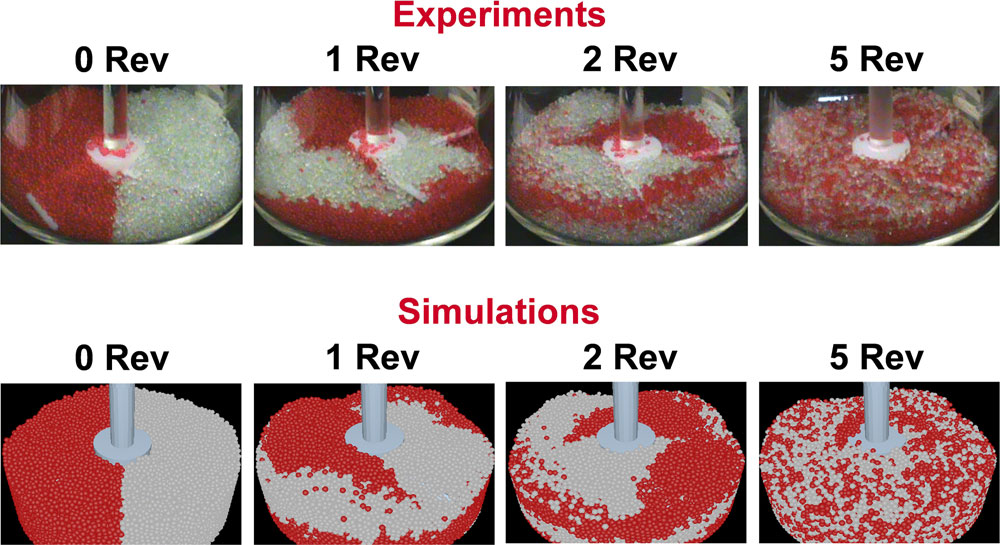
\includegraphics[width=0.65\textwidth]{images/introduction/drug_production.png}
	\end{center}
	% {\centerline{\includegraphics[scale=#2]{#1}}}
	% \vspace{-0.2cm}
	\label{fig:verlet_distance}
	\legend{Fonte: \alert{Citar fonte}}
	% \vspace{-1cm}
\end{figure}

Para partículas esféricas \(\particlei\) e \(\particlej\), a condição de vizinhança se escreve como
\begin{equation*}
	\norm{\positioni - \positionj} < \radiusi + \radiusj + \verletDistance,
\end{equation*}
como indicado na figura \ref{fig:verlet_distance}. 

\alert{Mostrar o conjunto vizinhança e dizer que, para o algoritmo de Verlet, esse conjunto é denominado de lista de Verlet}
\alert{Definir o deslocamento de Verlet como a distância \(\verletPosition\) entre a partícula e a sua posição quando a última lista de Verlet foi construída}

% Com isso, no instante \(t\), a vizinhança da \(i\)-ésima partícula é o conjunto
% \begin{equation*}
% 	\neighborhoodi\pqty{t} = \left\lbrace\particlej \,\suchThat\, \distanceij\pqty{t} < \radiusi + \radiusj + \verletDistance\right\rbrace,
% \end{equation*}
% em que \(\distanceij\) é a distância entre os centros das partículas \(i\) e \(j\).

Ao longo da simulação, porém, a movimentação das partículas faz com que sua vizinhança se altere, e assim é necessário reconstruir as listas de Verlet.

\subsection{Algoritmo \textit{link cell}}
\subsection{Algoritmo \textit{lattice}}

\section{Identificação de Contatos}

\section{Limitação do Passo de Tempo}

\alert{Ver \citeonline{bib:cundall1979} e \citeonline{bib:gomes2014}}

\alert{Explicar que o passo de tempo deve ser menor que um limite. Ver se essa seção é mesmo necessária.}

\section{Condições de Contorno e Restrições} \label{sec:boundary_condition}

\section{Outros Aspectos do Método}
\alert{Considerar, principalmente, \citeonline{bib:bicanic2007}. Essa seção deve falar que existem o estudo de fratura e fragmentação, abordagem para corpos deformáveis e esquemas de variação do passo de tempo}

\section{Acoplamento com Outros Métodos}
\alert{Falar aqui como o \DEM{} pode ser acoplado com CFD e FEM}